\subsection[Deep Learning]{\textit{Deep Learning}}

%\subsubsection[Training e test set]{Training e test set}

%\begin{frame}
%
%	\frametitle{Neural Networks}
%
%	\begin{figure}[!htbp]
%		\centering
%		\includegraphics[width=0.90\linewidth]{images/supervised/z_algorithms_neural_networks/nn.jpeg}
%		%\caption{}
%	\end{figure}
%
%\end{frame}

\begin{frame}

	\frametitle{Deep Learning}

	\begin{figure}[!htbp]
		\centering
		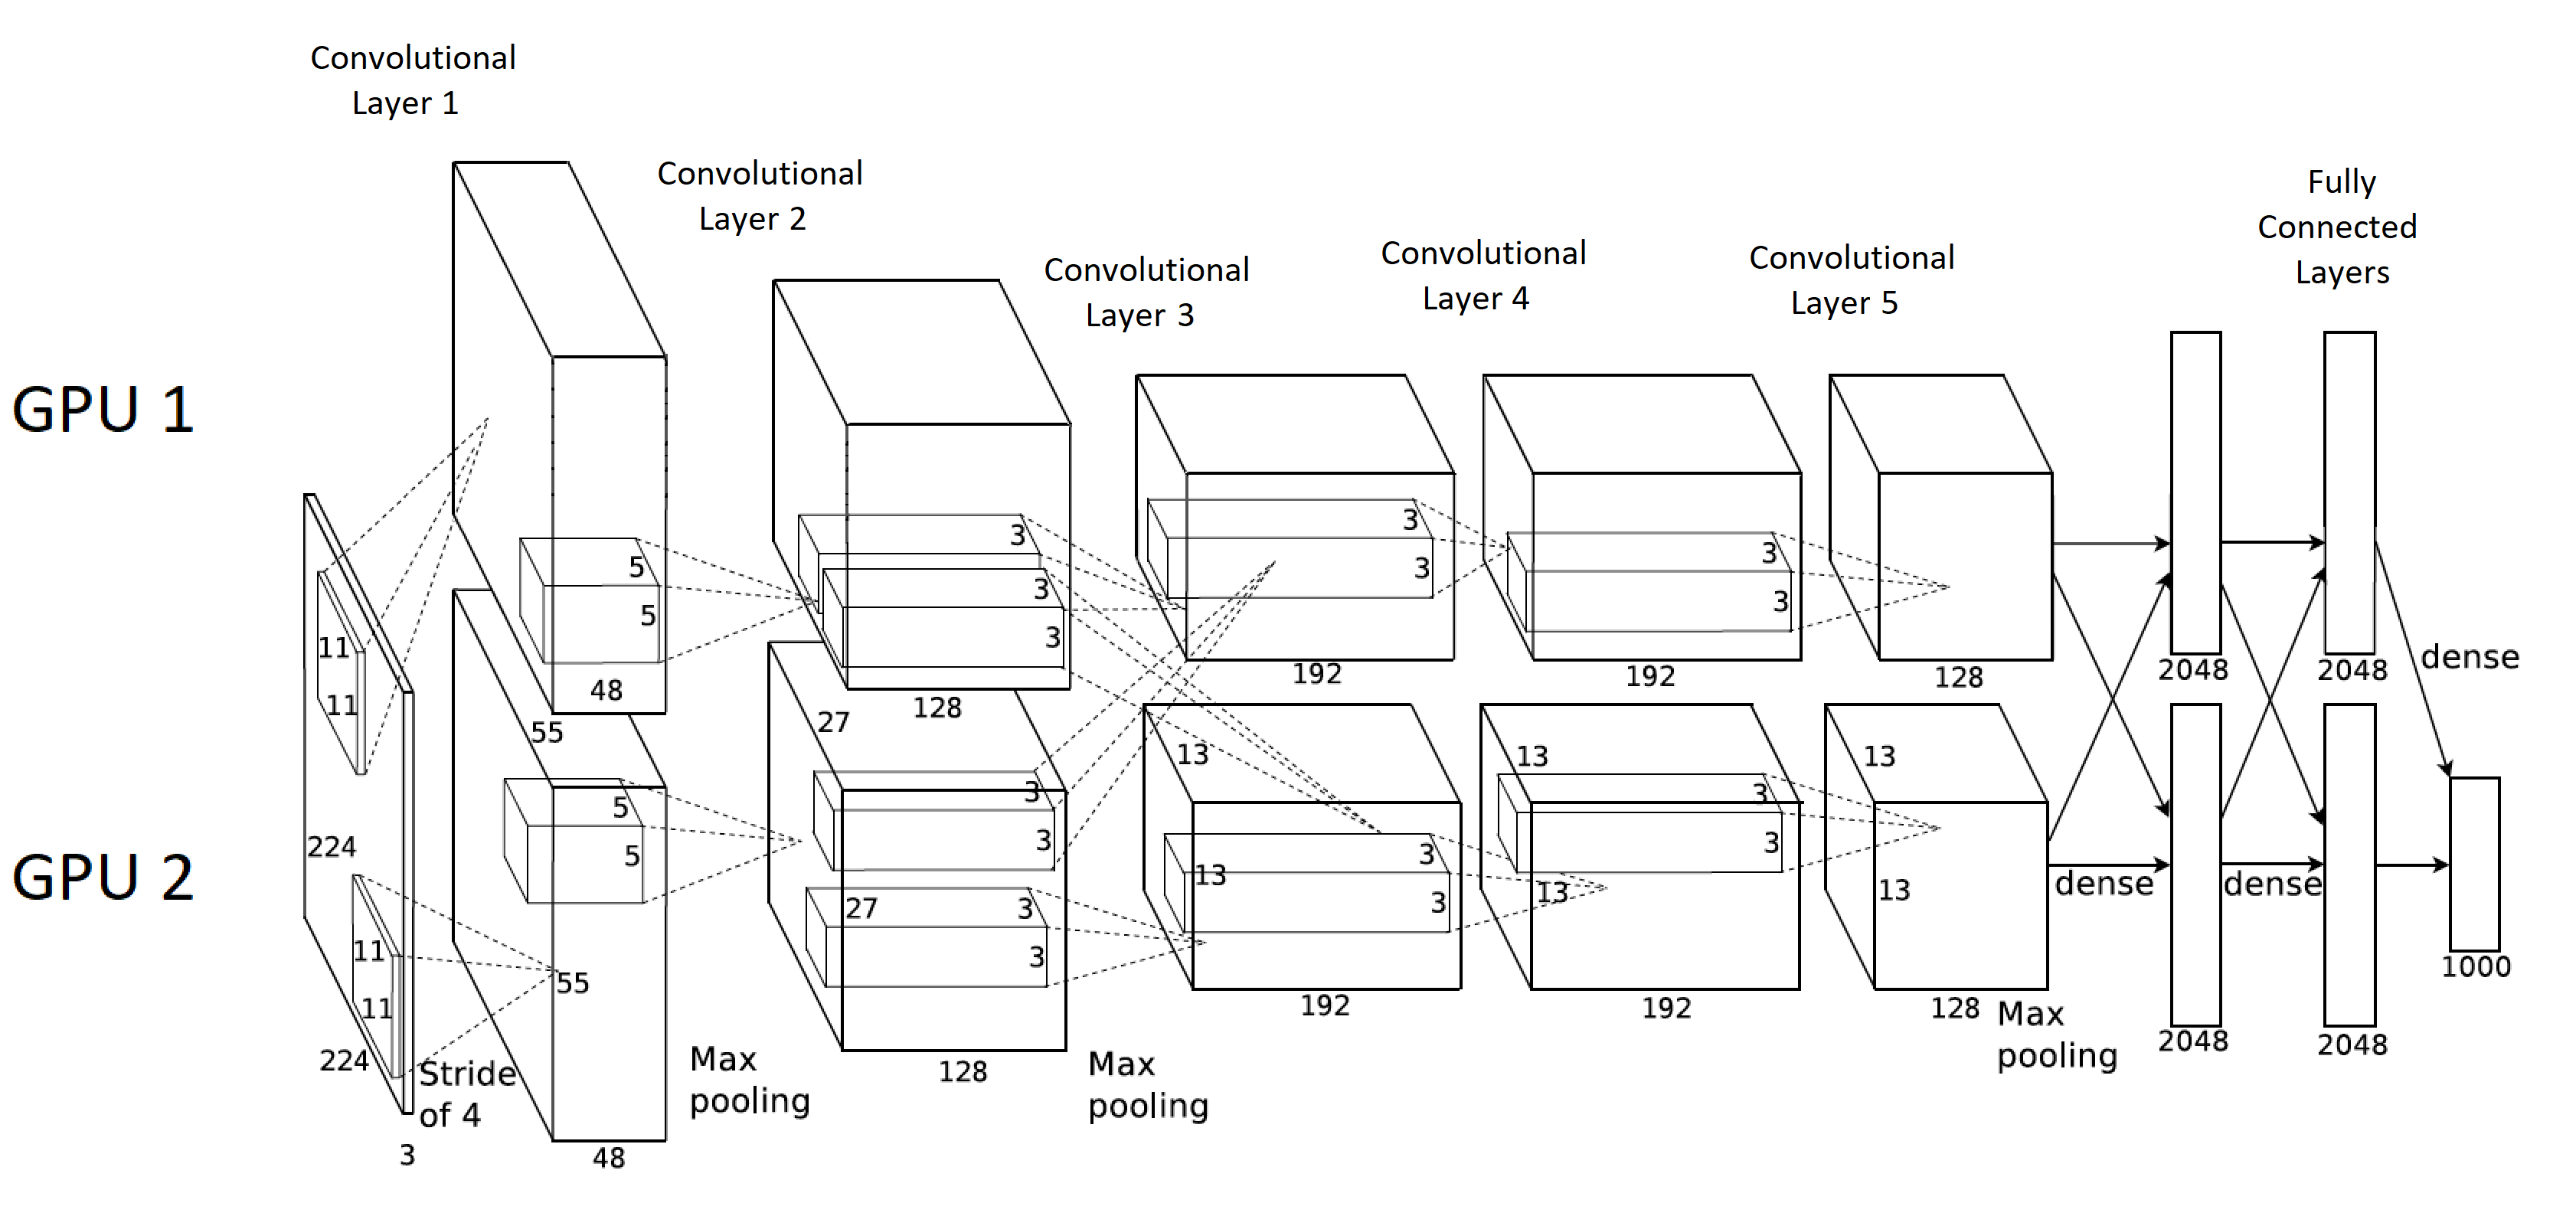
\includegraphics[width=1.0\linewidth]{images/supervised/z_algorithms_deep_learning/tensor_1.png}
		%\caption{}
	\end{figure}

\end{frame}


\subsubsection[Verso le Deep Neural Networks (DNN)]{Verso le Deep Neural Networks (DNN)}
\begin{frame}

	\frametitle{Deep Learning}

	Dopo la \textbf{backpropagation}, le successive innovazioni delle reti neurali portarono allo sviluppo del deep learning.
	\newlinedouble
	Per certe applicazioni, sono necessarie reti più estese e complesse (per apprendere feature complesse come le caratteristiche di una serie di immagini), il che porta al comparire di problemi come quello della \textbf{scomparsa del gradiente}.
	\newlinedouble
	Quando si addestra una grande rete, in effetti, l'errore si ridistribuisce fra i neuroni, favorendo i livelli più prossimi a quello di output. I livelli più lontani ricevono errori più piccoli, a volte troppo piccoli, il che rende l'addestramento più lento, se non impossibile. Sono stati ideati \textbf{nuovi sistemi per aggirare il problema} della scomparsa del gradiente: il risultato aiuta a realizzare reti più estese, ma il deep learning non è soltanto una questione di creare reti neurali con un numero più elevato di livelli e unità.
\end{frame}


\begin{frame}

	\frametitle{Deep Learning: feature engineering, convoluzioni e dropout}

	Nel deep learning ciò che è cambiato è qualcosa che riguarda strettamente la qualità del processamento dei dati, rispetto alle reti neurali meno profonde, facendo in modo che il paradigma del machine learning passasse dalla \textbf{creazione di feature} all'\textbf{apprendimento delle feature}.% (feature complesse create automaticamente sulla base di quelle effettive).
	\newlinedouble
	Visto che il riconoscimento delle immagini è pesantemente basato sulle reti neurali, il deep learning ha avuto una spinta importante grazie a un certo tipo di rete neurale, quella \textbf{convoluzionale}.
	\newlinedouble
	Infine, il \textbf{dropout} è un nuovo tipo di regolarizzazione particolarmente efficace con le DNN, che agisca rimuovendo temporaneamente e casualmente delle connessioni fra neuroni dai calcoli della rete. In questo modo, ne vengono temporaneamente rimosse alcune a caso, evitando che l'ottimizzazione, nel corso dell'addestramento, finisca con il dipendere da particolari connessioni che tendono a registrare informazioni troppo specifiche del dataset di addestramento.

\end{frame}

\begin{frame}

	\frametitle{Deep Learning: feature engineering, convoluzioni e dropout}

	\begin{figure}[!htbp]
		\centering
		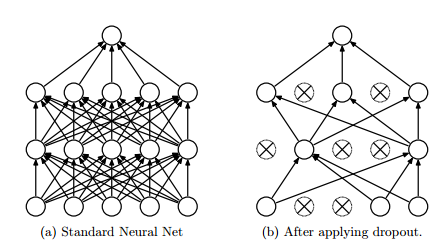
\includegraphics[width=0.9\linewidth]{images/supervised/z_algorithms_deep_learning/dropout.png}
		%\caption{}
	\end{figure}

\end{frame}


\subsubsection[Machine Learning vs Deep Learning]{Machine Learning vs Deep Learning}
\begin{frame}

	\frametitle{Machine Learning vs Deep Learning}

	\begin{figure}[!htbp]
		\centering
		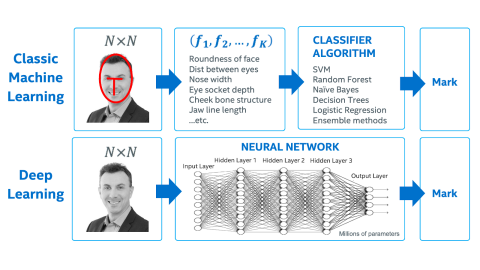
\includegraphics[width=1.0\linewidth]{images/supervised/z_algorithms_deep_learning/machine-vs-deep-learning-facial-recognition.png}
		%\caption{}
	\end{figure}

\end{frame}


\subsubsection[Correlazione e Convoluzione]{Correlazione e Convoluzione}
\begin{frame}

	\frametitle{Applicazione di un operatore locale a un'immagine}

%	\begin{block}{Applicazione di un operatore locale a un'immagine:}
		\begin{columns}
			\column{0.5\linewidth}
		  	\begin{enumerate}
				\item Definisci una maschera associata all'operatore
				\item Centra la maschera sul primo pixel dell'immagine
				\item Calcola la risposta dell'operatore come somma dei prodotti dei coefficienti della maschera e dei valori dei pixel dell'immagine
				\item Se tutti i pixel dell'immagine sono stati elaborati stop.\\	Altrimenti, sposta la maschera sul pixel successivo dell'immagine e vai a 3
			\end{enumerate}

			\column{0.5\linewidth}
			\begin{figure}[!htbp]
				\centering
				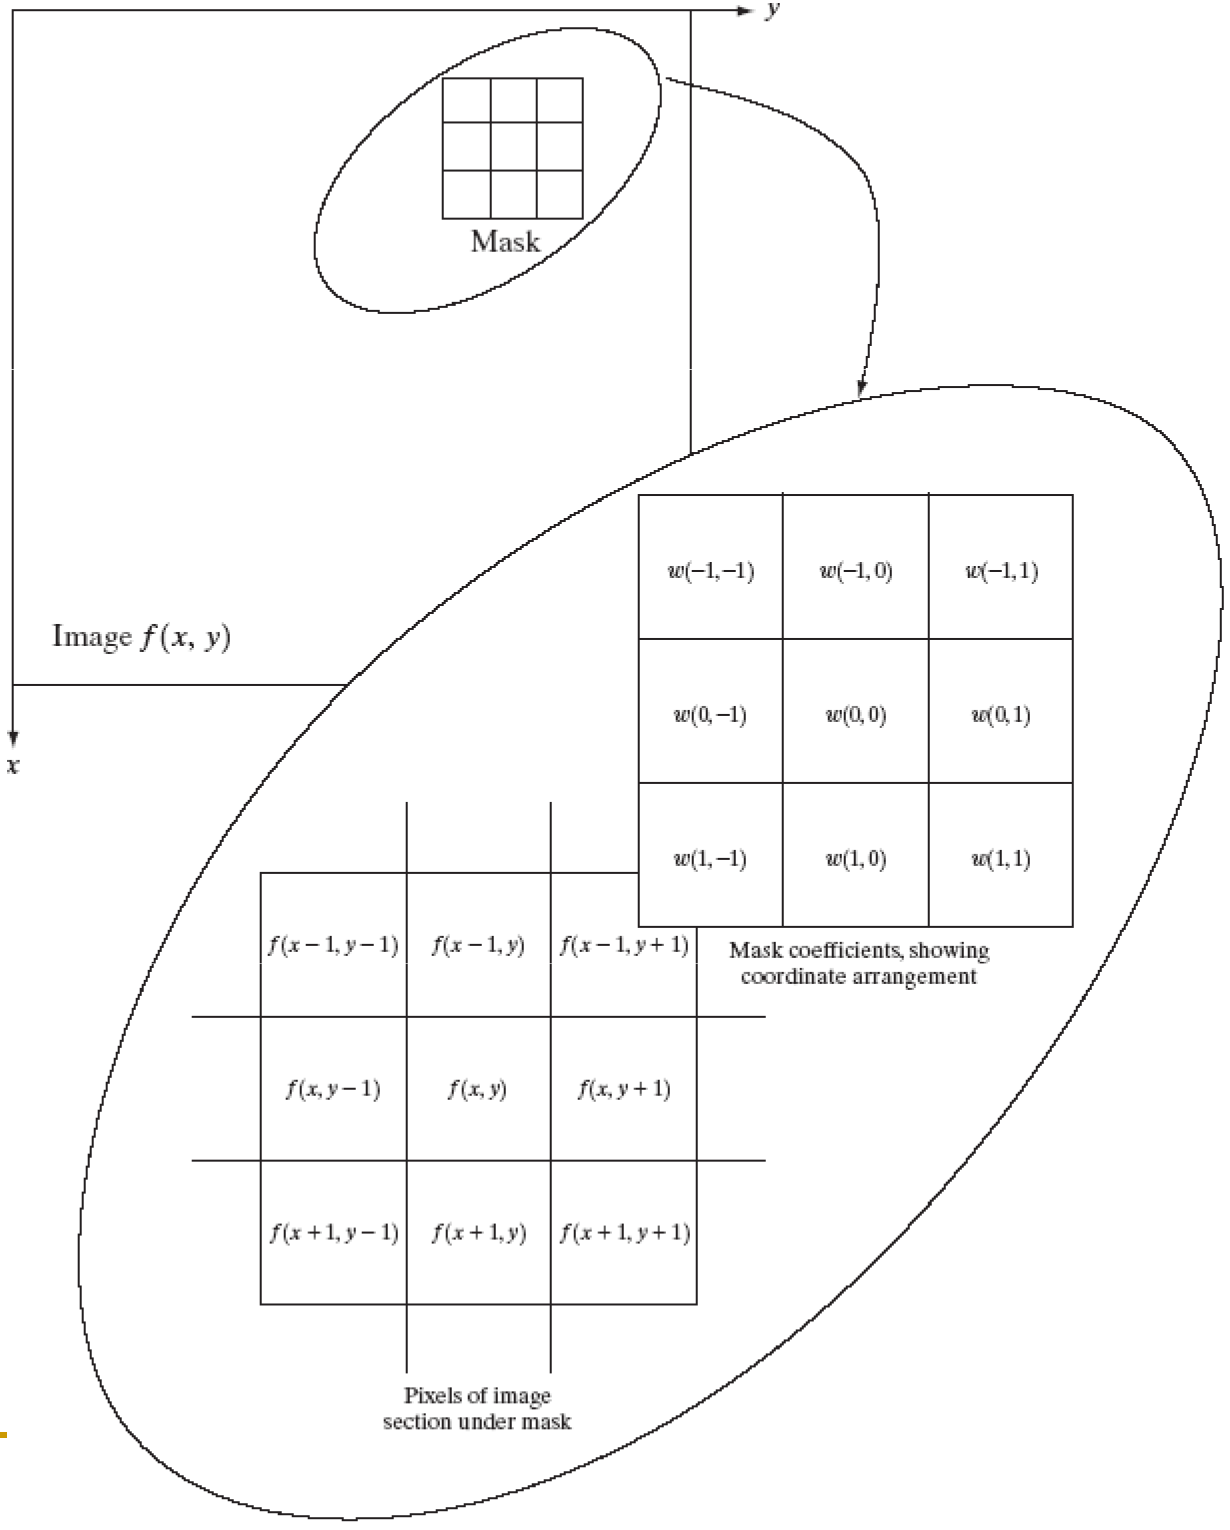
\includegraphics[width=0.95\linewidth]{images/supervised/z_algorithms_deep_learning/convolution_and_correlation_1.png}
				%\caption{}
			\end{figure}

		\end{columns}
%	\end{block}

\end{frame}


\begin{frame}

	\frametitle{Applicazione di un operatore locale a un'immagine}

%	\begin{block}{Applicazione di un operatore locale a un'immagine:}
		\begin{columns}
			\column{0.5\linewidth}
		  	Pertanto, la \textbf{risposta} dell'operatore locale $g(x, y)$
		  	può essere espressa come:
		  	$$g(x, y) = \sum_{i=-N}^{N} \sum_{j=-M}^{M} w(i, j) f(x+i, y+j)$$
		  	supponendo che la dimensione della maschera sia $(2N+1)*(2M+1)$

			\column{0.5\linewidth}
			\begin{figure}[!htbp]
				\centering
				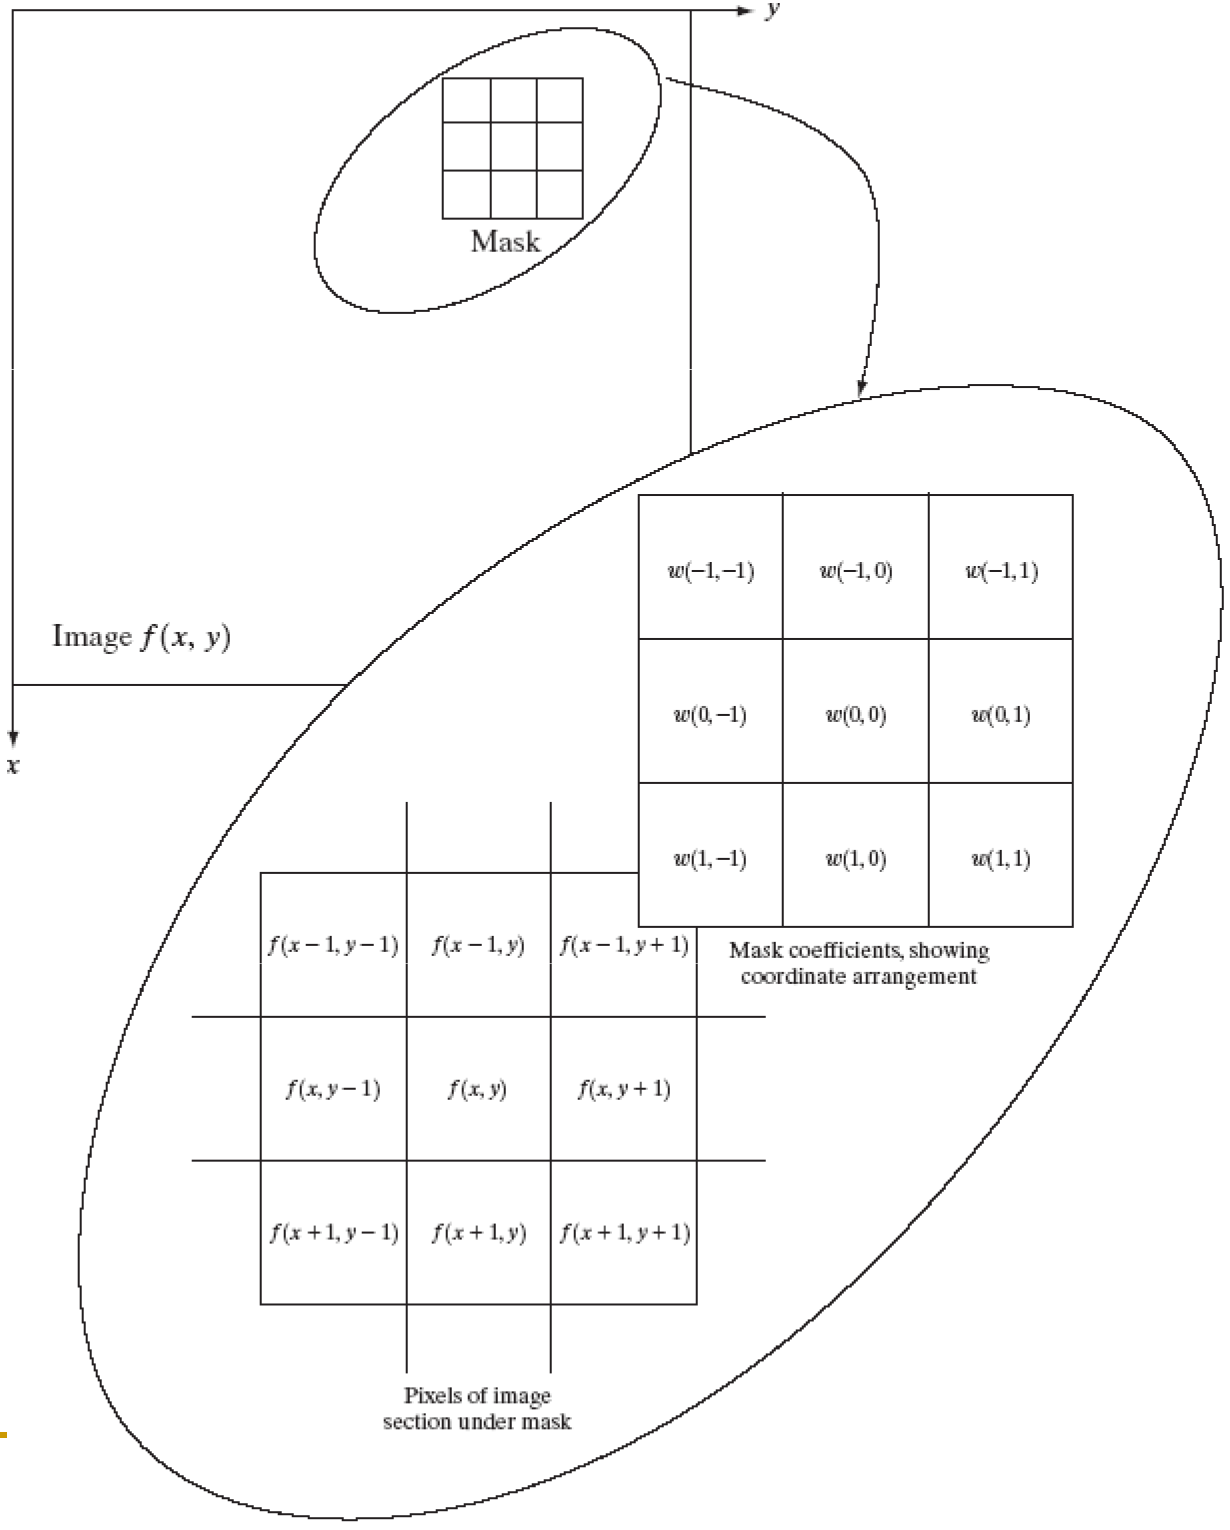
\includegraphics[width=0.95\linewidth]{images/supervised/z_algorithms_deep_learning/convolution_and_correlation_1.png}
				%\caption{}
			\end{figure}

		\end{columns}
%	\end{block}

\end{frame}


\begin{frame}

	\frametitle{Correlazione e Convoluzione}

	Distinguiamo tra:
	\begin{itemize}
		\item \textbf{Correlazione}:
			$$g(x, y) = w(x, y) \otimes f(x, y) = \sum_{i=-N}^{N} \sum_{j=-M}^{M} w(i, j) f(x+i, y+j)$$
		\item \textbf{Convoluzione}:
			$$g(x, y) = w(x, y) * f(x, y) = \sum_{i=-N}^{N} \sum_{j=-M}^{M} w(i, j) f(x-i, y-j)$$
	\end{itemize}

	\begin{tcolorbox}[colback=yellow!10,colframe=blue!40!black!60]
	  I segni negativi davanti agli indici incrementali alterano l'operazione ruotando il kernel di 180° prima della moltiplicazione pixel per pixel
	\end{tcolorbox}
\end{frame}


\begin{frame}

	\frametitle{Correlazione e Convoluzione}

	\begin{figure}[!htbp]
		\centering
		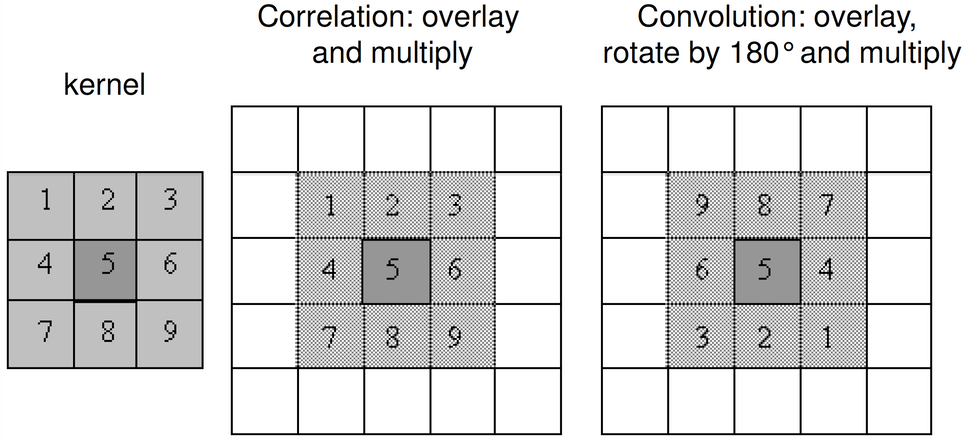
\includegraphics[width=0.8\linewidth]{images/supervised/z_algorithms_deep_learning/convolution_and_correlation_2.png}
		%\caption{}
	\end{figure}

	\begin{tcolorbox}[colback=yellow!10,colframe=blue!40!black!60]
	  Se il kernel è simmetrico rispetto a entrambi gli assi, la correlazione e la convoluzione producono lo stesso risultato
	\end{tcolorbox}

\end{frame}


\begin{frame}

	\frametitle{Correlazione e Convoluzione}

	Tuttavia, la convoluzione e la correlazione hanno proprietà diverse:
	\begin{itemize}
		\item \textbf{Convoluzione}:
			\begin{itemize}
				\item[--] è commutativa: $w * f = f * w$
				\item[--] è associativa: $w * (f * g) = (w * f) * g$
			\end{itemize}
		\item \textbf{Correlazione}:
			\begin{itemize}
				\item[--] non è commutativa: $w \otimes f \neq f \otimes w$
				\item[--] non è associativa: $w \otimes (f \otimes g) \neq (w \otimes f) \otimes g$
			\end{itemize}
	\end{itemize}
	\ \\
	Per questo nella elaborazione delle immagini e nelle architetture DNN è molto più comune trovare utilizzata la convoluzione piuttosto che la correlazione.
	\newlinedouble
	Più avanti vedremo un semplice esempio di come la convoluzione possa essere utilizzata all'interno di una DNN in un problema reale (MNIST: convolutional DNN).

\end{frame}


\begin{frame}

	\frametitle{Esempio, MNIST: il dataset, digits 28 x 28}

	\begin{figure}[!htbp]
		\centering
		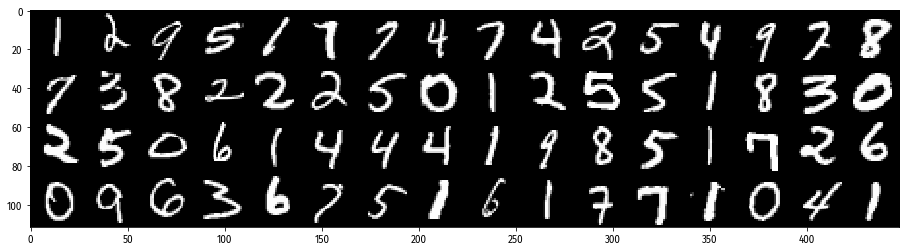
\includegraphics[width=1.0\linewidth]{images/supervised/z_algorithms_deep_learning/mnist.png}
		%\caption{}
	\end{figure}

\end{frame}


\begin{frame}

	\frametitle{Esempio, MNIST: rete neurale con 1 layer}

	\begin{figure}[!htbp]
		\centering
		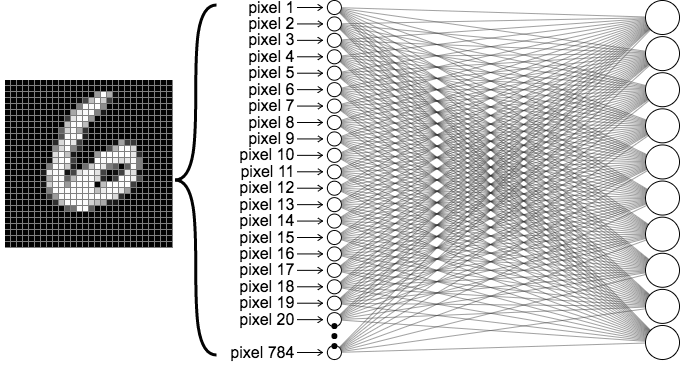
\includegraphics[width=1.0\linewidth]{images/supervised/z_algorithms_deep_learning/mnist_1layer.png}
		%\caption{}
	\end{figure}

\end{frame}


\begin{frame}

	\frametitle{Esempio, MNIST: rete neurale con 2 layer}

	\begin{figure}[!htbp]
		\centering
		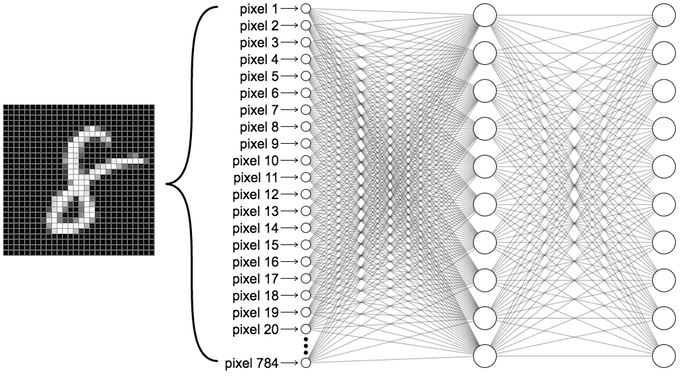
\includegraphics[width=1.0\linewidth]{images/supervised/z_algorithms_deep_learning/mnist_2layers.png}
		%\caption{}
	\end{figure}

\end{frame}


\begin{frame}

	\frametitle{Esempio, MNIST: rete neurale con 3 layer}

	%\begin{block}{}
		\centering
		\animategraphics[controls={play, step, stop}, height=7cm]{1.0}{images/supervised/z_algorithms_deep_learning/mnist_3layers/mnist_3layers-}{0}{17}
	%\end{block}

\end{frame}


\begin{frame}

	\frametitle{Esempio, MNIST: rete neurale con 3 layer}

	%\begin{block}{}
		\centering
		\animategraphics[controls={play, step, stop}, height=7cm]{2.0}{images/supervised/z_algorithms_deep_learning/nn-weights-biases/nn-weights-biases-}{0}{30}
	%\end{block}

\end{frame}


\begin{frame}

	\frametitle{Esempio, MNIST: rete neurale con 3 layer}

	\begin{figure}[!htbp]
		\centering
		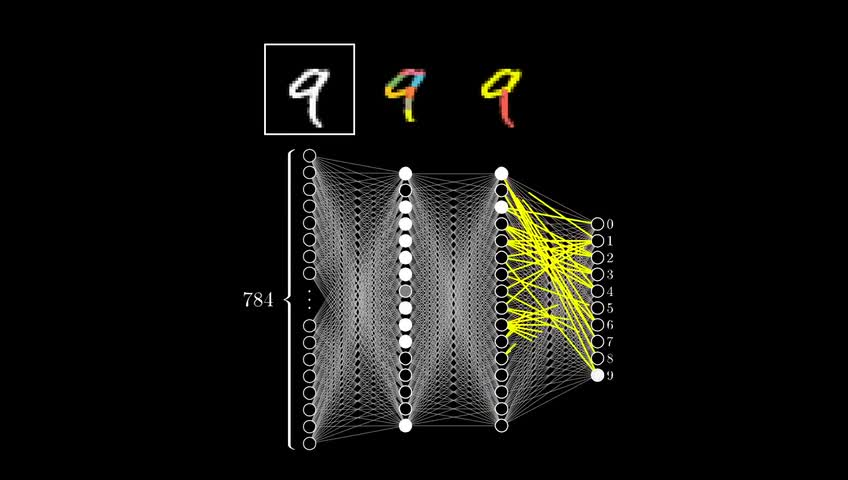
\includegraphics[width=1.0\linewidth]{images/supervised/z_algorithms_deep_learning/mnist_3layers_splits.jpg}
		%\caption{}
	\end{figure}


\end{frame}


\begin{frame}

	\frametitle{Esempio, MNIST: convolutional DNN}

	\begin{figure}[!htbp]
		\centering
		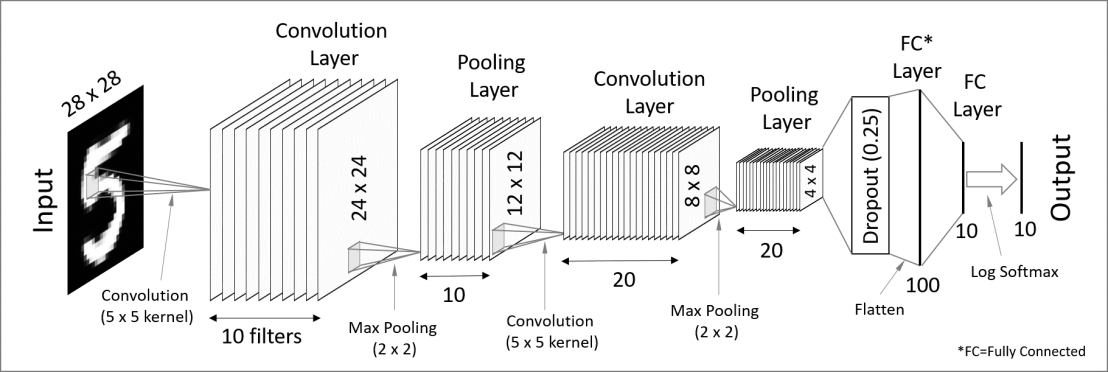
\includegraphics[width=1.0\linewidth]{images/supervised/z_algorithms_deep_learning/mnist_dnn.png}
		%\caption{}
	\end{figure}


\end{frame}


%\begin{frame}
%
%	\frametitle{DNN: l'esempio di MNIST, rete neurale con 3 layer}
%
%	\begin{figure}[!htbp]
%		\centering
%		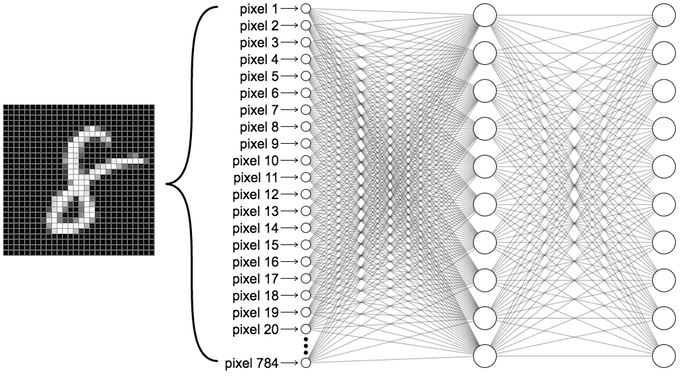
\includegraphics[width=1.0\linewidth]{images/supervised/z_algorithms_deep_learning/mnist_2layers.png}
%		%\caption{}
%	\end{figure}
%
%\end{frame}
